\chapter{Design and Implementation}

\section{Development Methodology}

\subsection{Development}
Since RAD was the chosen development methodology, the artefact was developed over several cycles.

\subsubsection{First Cycle}
In the first cycle the Mass-Spring model was implemented. Springs were implemented using the Hooke equation (Equation \ref{eq:hooke equation}) to calculate the internal spring force with linear damping as an additional internal force using Equation \ref{eq:spring damping}. Gravity, implemented as Equation \ref{eq:gravity}, was the only external force. Rendering of the cloth was also implemented.
\\Table \ref{tab:cycle 1 require} shows the requirements of the first development cycle.
\begin{table}[tp]
   \begin{minipage}{\textwidth}
      \begin{center}
         \begin{tabular}{c|c}
           Requirement & Type\\
           \hline
           Must model cloth using the Provot Mass-Spring model & Functional\\
           Must be able to render cloth to the screen & Functional\\
           Must be able to pin particles so they are unaffected by forces & Functional\\
           Must perform in real time& Non-functional\\
         \end{tabular}
      \end{center}
   \end{minipage}
   \caption{First cycle requirements}
   \label{tab:cycle 1 require}
\end{table}
\\\\Before designing this cycle, an initial investigation into the rendering component was carried out, as the choice between DirectX11 or OpenGL would affect the design of the system.
\\As this project is not concerned with rendering cloth, but simulating it, it was decided that the cloth would be rendered as a mesh of lines, representing the structural and shear springs (as in Figures \ref{fig:structural and shear} and \ref{fig:super-elasticity}). Since the positions of the particles, and therefore vertices, will change over time, a DirectX11 implementation would have to use a dynamic vertex buffer and remap the vertex data every frame. This is not an issue in OpenGL, since it is possible to draw vertices directly with the glVertex3f function. It was unknown by the author what the cost of this remapping would be so simple OpenGL and DirectX11 implementations were created and their performance compared. For a 500 by 500 mesh, the OpenGL implementation rendered the structural and shear springs at 80FPS and the DirectX11 version at 450FPS. Hence, DirectX11 was chosen as the rendering language. It should be noted that the OpenGL implementation was very naive, due to the author's inexperience, and this is most likely the reason for the poor performance. It is probable that a more robust implementation, using more advanced features, would perform much more closely to the DirectX11 implementation.
\\\\The initial design can be seen in Fig \ref{fig:phase1 initial}; the rendering component, constructors, accessors and mutators have been excluded for brevity. 
\\Since DirectX11 was the rendering language, DirectXMath types were used for the key variables in the Particle class. This gives performance gains over manually implementing a 3-dimensional vector and functions, as the functions that operate on DirectXMath types are compiled into SIMD instructions, allowing the calculations to be completed in less CPU cycles.
\\\\During implementation, the initial design had to be adapted as a result of performance concerns. 
\\Firstly the std::vector was replaced with dynamically allocated arrays in the Cloth class. Iterating though the vector to calculate the spring forces proved prohibitively expensive for meshes over a certain size, even calcSpringForce was an empty function; a 100 by 100 mesh was the largest mesh that supported real time frame rates, running at 40FPS. Switching to arrays gave a 4x FPS increase, for the same mesh size, and a 2x increase in the maximum real time mesh size.
\\Secondly, XMVECTORs were used in place of XMFLOAT3s in the Particle class. XMFLOAT3s must be converted into XMVECTORs using XMLoadFloat3 in order to be able to use the DirectXMath vector functions. Therefore, the position and velocity of every particle had to be converted every frame in order to implement Equations \ref{eq:hooke equation} and \ref{eq:spring damping}. Through profiling, it was found that this conversion was the most expensive part of calcSpringForce and so XMVECTORs were used instead, giving performance gains of 40FPS for a 50 by 50 mesh. Changing the accessors and mutators in Particle to return and pass by reference improved performance slightly also, giving gains of roughly 5FPS.
\\\\The final design of the first development cycle can be seen in Fig \ref{fig:phase1}

\subsubsection{Second Cycle}
During the second development cycle the model developed in the first cycle was adapted to use different integration methods. The explicit Euler and Verlet integrators were implemented as described in \ref{sec:explicit}. Wind was also added as an additional external force.

\subsubsection{Third Cycle}
In the final development cycle the fourth order Runge-Kutta and implicit Euler integrators were implemented.

\section{Testing Plan}

\subsection{Test Data}
To evaluate the performance impact of different integration method a number of data points will be captured from the simulation
\begin{itemize}
\item{Simulation frame rate. This will be affected by the cost and frequency of the integration calculations and is essential to capture to determine if the simulation is running in real time}
\item{Average time spent on integration calculations. Extracting this allows investigations into the affect of more expensive, but less frequent, integrators}
\item{Time taken to reach the equilibrium point. The equilibrium point is defined as the point at which there is close to zero total force for all particles, i.e. the external and internal forces are balanced. \textcite{Wang2009a} have shown that using higher order Runge-Kutta integrators reduces the time taken to reach equilibrium and thus, extracting this data will allow comparisons with their results}
\end{itemize}
In addition, the average time spent updating and rendering the cloth will also be extracted, in order to gain a better understanding of where the time each frame is spent.

\subsection{Test Parameters}


\section{System Requirements}
\label{sec:require}
Before proceeding with the design and implementation of any software project it is important to define the requirements of the system to be developed. The requirements of a system define what the system must be able to do and are normally split into functional and non-functional requirements. Functional requirements of a system specify the explicit behaviour of the system and non-functional requirements specify other properties of the system that aren't explicitly related to the functionality, e.g. performance, file types supported etc.
\\In a professional software engineering environment the requirements gathering process would be conducted with the end user of the system, in order to ensure that what is developed matches what the end users actually want, and not what the developers think they might want. In this situation, a variety of requirement gathering techniques would be employed, some of which may include
\begin{itemize}
  \item{Document analysis; analysing any existing documents the end users currently use. This can help to establish the structure of database tables, or simply the datatypes the system should use}
  \item{Interviews. By interviewing end users, it is easy to get a list of what they want as well as an idea on how the system currently works}
  \item{Observation. By observing the current system, an idea of the flow of data etc. can be gathered}
  \item{Research. Research into the technologies available, or other similar solutions, can be a key factor in specifying a system}
\end{itemize}
Due to the nature of the project there is no specific end user, so the requirements were based on the research described in the previous section.

\subsection{Functional Requirements}
\begin{itemize}
  \item{The system must be able to play Connect 4 in The Arena as effectively as possible} 
  \item{The system must be able to optimise any unconstrained real valued maximisation or minimisation problem}
  \item{The system must optimise within the bounds defined by the problem only}
  \item{The system must implement the genetic, evolution strategies and particle swarm optimisation algorithms as described in the previous section}
  \item{The genetic and evolution strategies algorithms must be implemented supporting a number of the different selection and recombination methods described in the previous section}
  \item{The state of the system must be able to be written to and loaded from a file}
  \item{The system must store the fitness of each individual at each generation, and must allow this data to be plotted on a scatter graph}
\end{itemize}

\subsection{Non-functional Requirements}
\begin{itemize}
  \item{The parameters of the algorithms must be easily changeable} 
  \item{The system must allow new problems to be defined as easily as possible} 
  \item{The system must allow problem specific stopping criteria to be easily defined}
  \item{The system must allow new binary or real value coded population based algorithms to be added easily}
  \item{The system must be fully documented using JavaDoc}
  \item{The system must be machine and operating system independent}
\end{itemize}

\section{Development Methodology}
Using a software development methodology helps to keep any large scale development project in check. Development methodologies split development into a number of phases, which build on top of each other and guide the development of the software. Typical phases in a development methodology are analysis, design, implementation and testing.
\\The primary development methodology chosen for this project was phased development. In this methodology, the system is developed in phases of design, implementation and testing, with each phase building on the previous one, as shown by figure \ref{fig:phased}\cite{phased}. The use of this methodology is supported by the project's first and second aims. These aims can be used to split the project into two developmental phases; first, to develop a generic optimisation library and second to adapt this library to The Arena.
\begin{figure}[tp]
   \begin{center}
     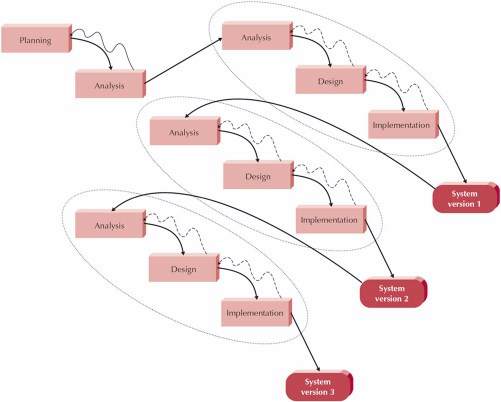
\includegraphics{Figures/phased}
   \end{center}
   \caption{Phased development methodology}
   \label{fig:phased}
\end{figure}